\documentclass[tikz,border=12pt]{standalone}
\usepackage[T1]{fontenc}
\usepackage{mathpazo}
\usepackage{amsmath,amssymb}
\usetikzlibrary{arrows.meta, positioning, calc, fit, decorations.pathreplacing}
\definecolor{stblue}{HTML}{7B97AD}
\definecolor{rwgold}{HTML}{B8995E}
\definecolor{sage}{HTML}{7A9A7E}
\definecolor{dkbrown}{HTML}{3D3530}
\definecolor{wmgray}{HTML}{7B7067}
\definecolor{cream}{HTML}{F9F6F0}
\definecolor{border}{HTML}{D4C9B8}
\definecolor{terracotta}{HTML}{C47A6A}
\definecolor{lavender}{HTML}{907EA0}

\begin{document}
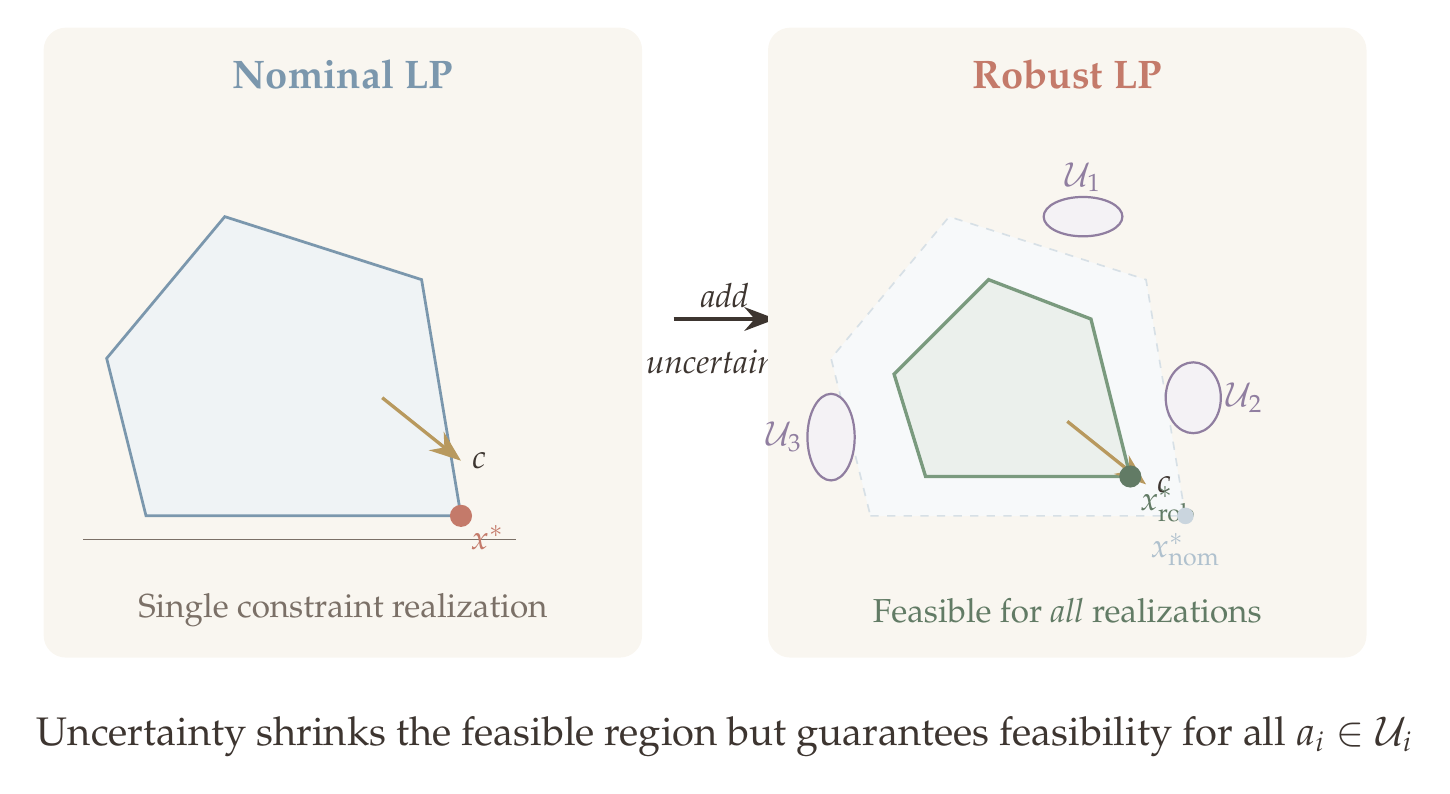
\begin{tikzpicture}[
    >={Stealth[length=4mm, width=3mm]},
    every node/.style={text=dkbrown},
  ]

  % ===== LEFT PANEL: Nominal LP =====
  \begin{scope}[shift={(0,0)}]
    % Background
    \fill[cream, rounded corners=8pt] (-0.8,-1.8) rectangle (6.8,6.2);

    % Title
    \node[font=\Large\bfseries, text=stblue] at (3.0,5.6) {Nominal LP};

    % Feasible region (polygon)
    \fill[stblue!12] (0.5,0) -- (4.5,0) -- (4,3) -- (1.5,3.8) -- (0,2) -- cycle;
    \draw[stblue, line width=1pt] (0.5,0) -- (4.5,0) -- (4,3) -- (1.5,3.8) -- (0,2) -- cycle;

    % Constraint lines extending beyond the polygon
    \draw[wmgray, line width=0.6pt] (-0.3,-0.3) -- (5.2,-0.3);

    % Objective direction arrow
    \draw[->, rwgold, line width=1.2pt] (3.5,1.5) -- (4.5,0.7)
      node[right, font=\large] {$c$};

    % Optimal point
    \fill[terracotta] (4.5,0) circle (4pt);
    \node[font=\large, terracotta, below right] at (4.5,0) {$x^*$};

    % Label
    \node[font=\large, text=wmgray, align=center] at (3.0,-1.2)
      {Single constraint realization};
  \end{scope}

  % ===== Arrow between panels =====
  \draw[->, dkbrown, line width=1.5pt] (7.2,2.5) -- (8.5,2.5)
    node[midway, above, font=\large\itshape] {add};
  \node[font=\large\itshape, text=dkbrown] at (7.85,1.9) {uncertainty};

  % ===== RIGHT PANEL: Robust LP =====
  \begin{scope}[shift={(9.2,0)}]
    % Background
    \fill[cream, rounded corners=8pt] (-0.8,-1.8) rectangle (6.8,6.2);

    % Title
    \node[font=\Large\bfseries, text=terracotta] at (3.0,5.6) {Robust LP};

    % Nominal feasible region (faded)
    \fill[stblue!6] (0.5,0) -- (4.5,0) -- (4,3) -- (1.5,3.8) -- (0,2) -- cycle;
    \draw[stblue!30, line width=0.6pt, dashed]
      (0.5,0) -- (4.5,0) -- (4,3) -- (1.5,3.8) -- (0,2) -- cycle;

    % Uncertainty ellipses around constraint lines
    \fill[lavender!10] (3.2,3.8) ellipse (0.5 and 0.25);
    \draw[lavender, line width=0.8pt] (3.2,3.8) ellipse (0.5 and 0.25);
    \node[font=\large, lavender] at (3.2,4.3) {$\mathcal{U}_1$};

    \fill[lavender!10] (4.6,1.5) ellipse (0.35 and 0.45);
    \draw[lavender, line width=0.8pt] (4.6,1.5) ellipse (0.35 and 0.45);
    \node[font=\large, lavender] at (5.25,1.5) {$\mathcal{U}_2$};

    \fill[lavender!10] (0.0,1.0) ellipse (0.3 and 0.55);
    \draw[lavender, line width=0.8pt] (0.0,1.0) ellipse (0.3 and 0.55);
    \node[font=\large, lavender] at (-0.6,1.0) {$\mathcal{U}_3$};

    % Robust feasible region (smaller, solid)
    \fill[sage!15] (1.2,0.5) -- (3.8,0.5) -- (3.3,2.5) -- (2.0,3.0) -- (0.8,1.8) -- cycle;
    \draw[sage, line width=1.2pt] (1.2,0.5) -- (3.8,0.5) -- (3.3,2.5) -- (2.0,3.0) -- (0.8,1.8) -- cycle;

    % Objective direction arrow
    \draw[->, rwgold, line width=1.2pt] (3.0,1.2) -- (4.0,0.4)
      node[right, font=\large] {$c$};

    % Robust optimal point
    \fill[sage!80!black] (3.8,0.5) circle (4pt);
    \node[font=\large, sage!80!black, below right] at (3.8,0.5) {$x^*_{\text{rob}}$};

    % Nominal optimal (faded)
    \fill[stblue!40] (4.5,0) circle (3pt);
    \node[font=\large, stblue!60, below] at (4.5,-0.1) {$x^*_{\text{nom}}$};

    % Labels
    \node[font=\large, text=sage!80!black, align=center] at (3.0,-1.2)
      {Feasible for \emph{all} realizations};
  \end{scope}

  % ===== Bottom annotation =====
  \node[font=\Large, text=dkbrown, align=center] at (7.85,-2.8)
    {Uncertainty shrinks the feasible region but guarantees feasibility for all $a_i \in \mathcal{U}_i$};

\end{tikzpicture}
\end{document}
